\documentclass{beamer}
\beamertemplatenavigationsymbolsempty
\usecolortheme{beaver}
\setbeamertemplate{blocks}[rounded=true, shadow=true]
\setbeamertemplate{footline}[page number]
%
\usepackage[utf8]{inputenc}
\usepackage[english,russian]{babel}
\usepackage{amssymb,amsfonts,amsmath,mathtext}
\usepackage{subfig}
\usepackage[all]{xy} % xy package for diagrams
\usepackage{array}
\usepackage{multicol} % many columns in slide
\usepackage{hyperref} % urls
\usepackage{hhline} %tables
\usepackage{comment} %comments
% Your figures are here:
\graphicspath{ {../figures/} }

%----------------------------------------------------------------------------------------------------------

\title[\hbox to 56mm{Дистилляция знаний в глубоких сетях}]{Дистилляция знаний в глубоких сетях и выравнивание структур моделей}
\author[М.\,С.~Олейник]{Михаил Сергеевич Олейник}
\institute{Московский физико-технический институт}
\date{\footnotesize
\par\smallskip\emph{Курс:} Моя первая научная статья
\par\smallskip\emph{Консультант:} М. Горпинич
\par\bigskip\small 2023}

%----------------------------------------------------------------------------------------------------------
\begin{document}
%----------------------------------------------------------------------------------------------------------

\begin{frame}

    %\thispagestyle{empty}
    \maketitle

\end{frame}

%-----------------------------------------------------------------------------------------------------

\begin{frame}{Предлагаемый подход}

    \begin{columns}[c]
        \column{0.4\textwidth}
        \begin{figure}
            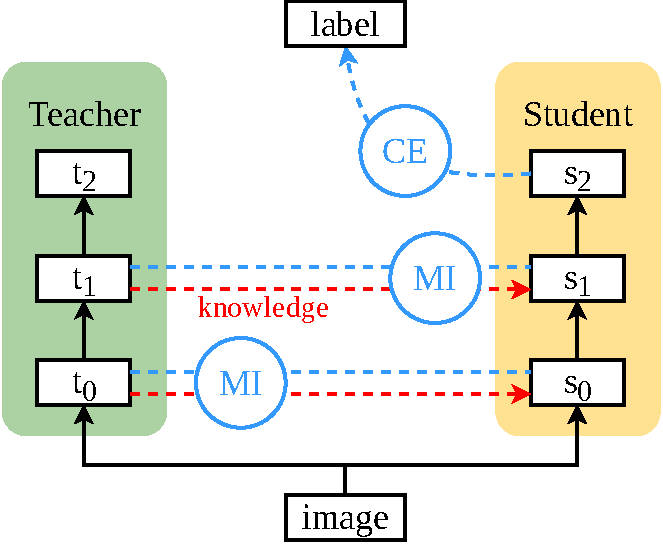
\includegraphics[width=1.0\textwidth]{ahn_diagram.pdf}
            \caption{Базовый метод}
        \end{figure}

        \column{0.4\textwidth}
        \begin{figure}
            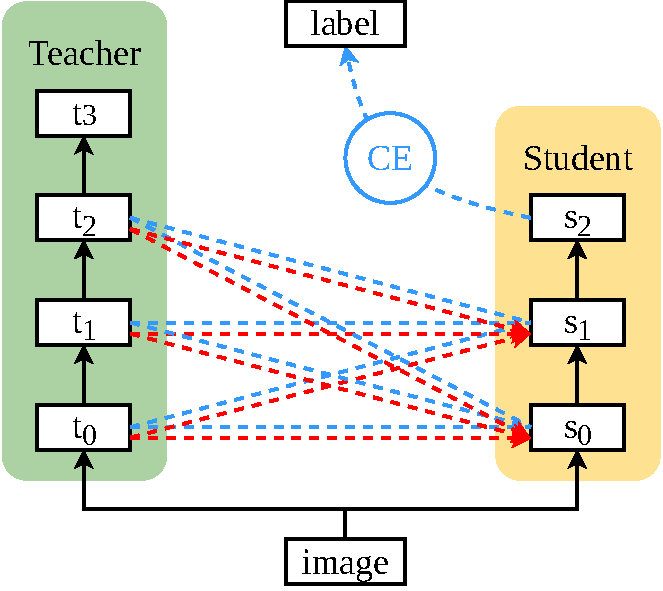
\includegraphics[width=1.0\textwidth]{our_diagram.pdf}
            \caption{Предлагаемый метод}
        \end{figure}
    \end{columns}

    \begin{columns}[c]
        \column{0.6\textwidth}
        \begin{equation}
            \mathcal{L} = \beta \mathcal{L}_\text{CE} - (1 - \beta){\sum_{i, j=1}^{T, S}\lambda_{i, j}I(t_{i}, s_{j})}
        \end{equation}
        \vspace*{-\baselineskip}\setlength\belowdisplayshortskip{0pt}
        \begin{equation}
            \forall j \hookrightarrow  \sum_{i=1}^{T}\lambda_{i, j} = 1
        \end{equation}

        \column{0.4\textwidth}
        $T, S$ - количество слоёв учителя и ученика,

        $I(t_{i}, s_{j})$ - взаимная информация,

        $\beta$ и $\lambda_{i, j}$ --- гиперпараметры.
    \end{columns}

\end{frame}

%----------------------------------------------------------------------------------------------------------

\begin{frame}{Взаимная информация}
    Метод вариации нижней границы:
    \begin{equation}
        I(t, s) = H(t) - H(t|s) \geq  H(t) + E_{t,s}[\log{q(t|s)}].
    \end{equation}
    Как будет выглядеть вариационное распределение?
    \begin{multline}
        -\log{q(t|s)} = -\sum_{c=1}^{C}  \sum_{h=1}^{H} \sum_{w=1}^{W} \log{q(t_{c,h,w}|s)} = \\
        = \sum_{c=1}^{C}  \sum_{h=1}^{H} \sum_{w=1}^{W} \log{\sigma_c} + \frac{(t_{c,h,w} - \mu_{c,h,w}(s))^2}{2\sigma_c^2} + constant.
    \end{multline}
    Обучаемые параметры скрываются здесь:
    $$\sigma^2_c = \log{(1 + e^{\alpha_c})} + \epsilon$$
    $$\mu_{c,h,w}(s) = \mu(s)_{c,h,w}$$
\end{frame}

%----------------------------------------------------------------------------------------------------------

\begin{frame}{Эксперимент}
    \begin{columns}[c]
        \column{0.4\textwidth}
        \textbf{Выборка}: CIFAR10.

        \textbf{Модели}: 3 conv, 2 linear.

        \textbf{Метрика}: accuracy.

        \column{0.55\textwidth}
        \begin{figure}
            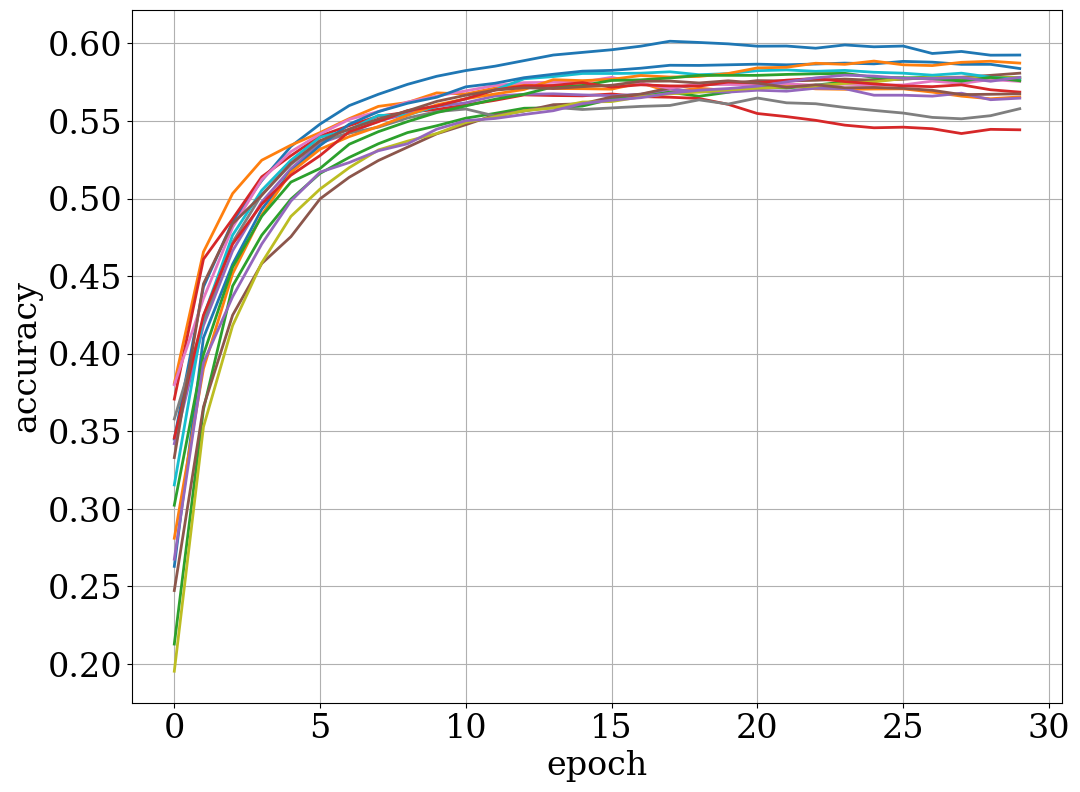
\includegraphics[width=1.0\textwidth]{distill_epoch_accuracy.png}
            \caption{Точность от эпохи при дистилляции каждый с каждым}
        \end{figure}
    \end{columns}

    \begin{table}[]
        \begin{tabular}{|l|l|l|l|l|}
            \hline
            Дистилляция & ---  & Хинтона & попарная  & каждый с каждым \\ \hline
            Учитель     & 0.58 & ---     & ---       & ---             \\ \hline
            Ученик      & 0.54 & 0.56    & 0.58-0.59 & 0.58-0.59       \\ \hline
        \end{tabular}
        \caption{Сравнение качества моделей на тестовой выборке}
    \end{table}
\end{frame}

%----------------------------------------------------------------------------------------------------------

\begin{frame}{Ограничения на коэффициенты}
    \begin{figure}[H]
        \begin{minipage}[h]{0.35\linewidth}
            \center{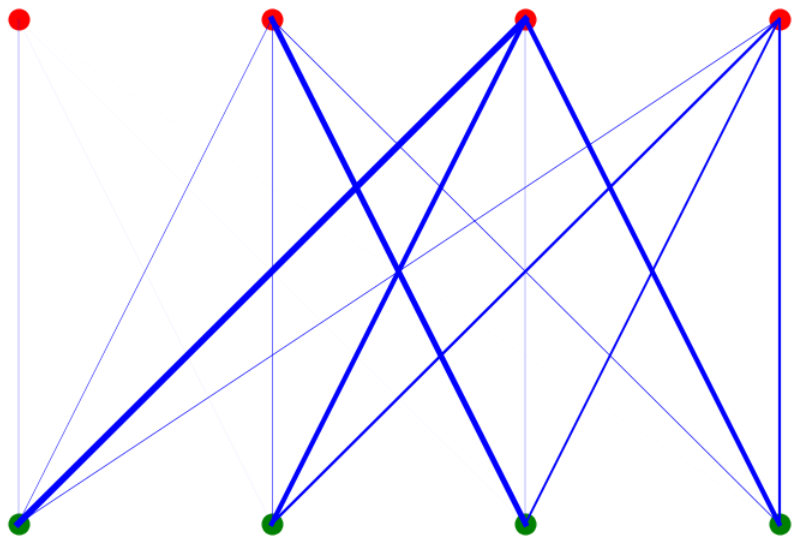
\includegraphics[width=1\linewidth]{connections_1}} a) \\
        \end{minipage}
        \hfill
        \begin{minipage}[h]{0.35\linewidth}
            \center{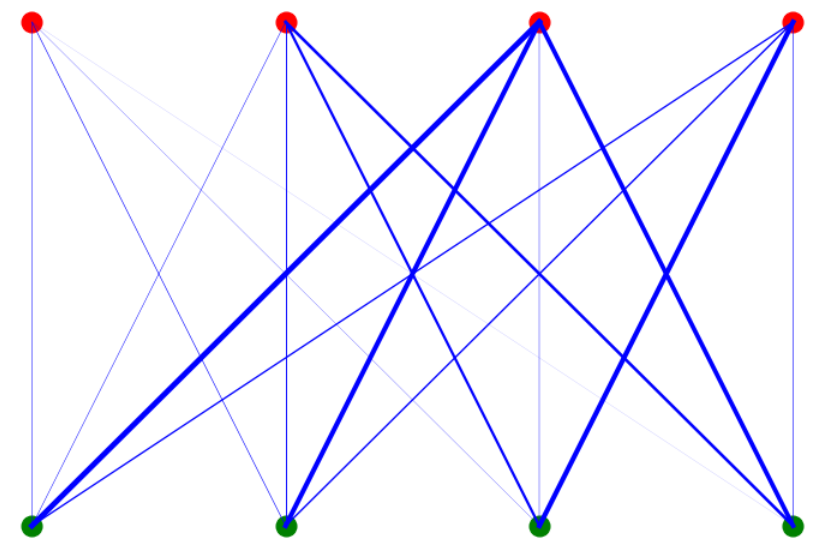
\includegraphics[width=1\linewidth]{connections_2}} b) \\
        \end{minipage}
        \vfill
        \begin{minipage}[h]{0.35\linewidth}
            \center{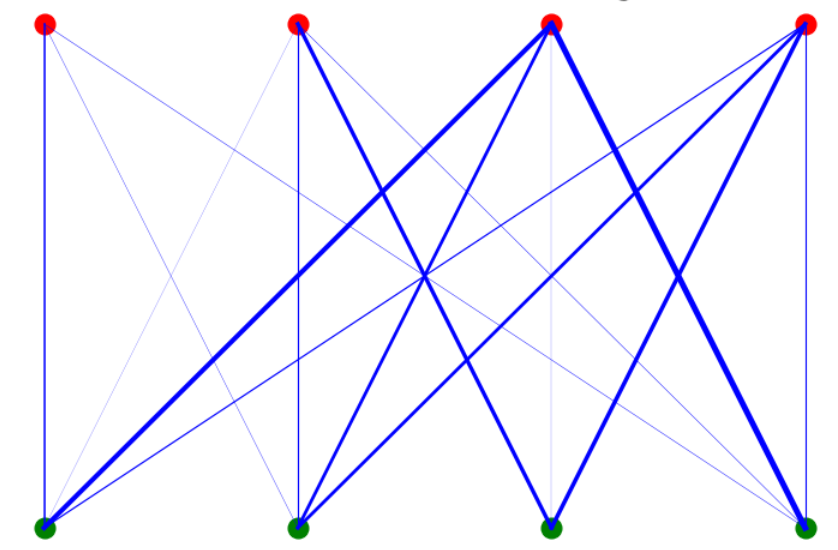
\includegraphics[width=1\linewidth]{connections_3}} c) \\
        \end{minipage}
        \hfill
        \begin{minipage}[h]{0.35\linewidth}
            \center{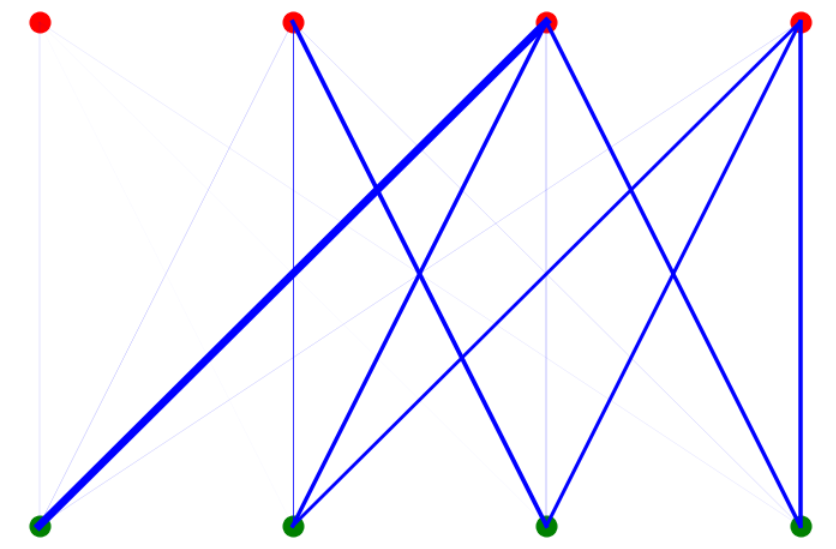
\includegraphics[width=1\linewidth]{connections_4}} d) \\
        \end{minipage}
        \caption{Иллюстрация коэффициентов у четырех лучших моделей по качеству. Зелёные точки --- слои ученика, красные --- слои учителя. Чем толще линия, тем больше коэффициент у соответствующей связи.}
    \end{figure}
\end{frame}

%----------------------------------------------------------------------------------------------------------

\begin{frame}{Промежуточные выводы}
    \begin{itemize}
        \item Между учителем и учеником мало различий, не можем увидеть разницу в качестве у разных подходов.
              Пробуем с учителем побольше.
        \item Какие-то закономерности с коэффициентами присутствуют. Утверждать рано, продолжаем изучать.
    \end{itemize}
\end{frame}

%----------------------------------------------------------------------------------------------------------
\end{document}